\chapter{製作歷程}

\section{移動方式}
%=--------------------移動方式----------------------=%
在原有的設計上,將自動移動改成了使用鍵盤操控\\
w向上,a向左,s向下,d向右\\
觸發不同條件來改變兩joint的速度達到變動方向的效果
\begin{figure}[hbt!]
\begin{center}
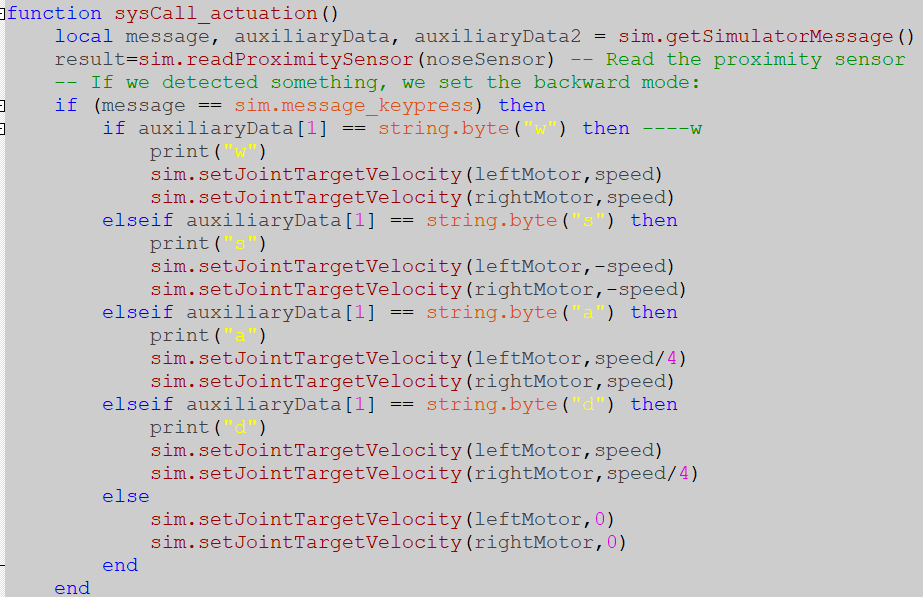
\includegraphics[width=16cm]{lua move}
\caption{\Large lua move }\label{ lua move}
\end{center}
\end{figure} 
\section{重製位置}
%=--------------------重製位置----------------------=%
添加了只要觸發特定條件就能使bubbleRob 雙輪車回到原位\\
先記錄初始位置
\begin{figure}[hbt!]
\begin{center}
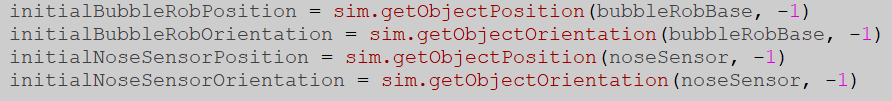
\includegraphics[width=16cm]{紀錄初始位置}
\caption{\Large 紀錄初始位置 }\label{紀錄初始位置}
\end{center}
\end{figure} 
\qquad \\
在觸發特定條件時使用來達成重製效果
\begin{figure}[hbt!]
\begin{center}
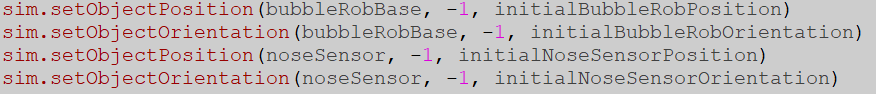
\includegraphics[width=16cm]{重製位置}
\caption{\Large 重製位置 }\label{重製位置}
\end{center}
\end{figure} 
\section{記分板與計時}
%=--------------------記分板與計時----------------------=%
增加倒數計時與分數的面板,遊戲開始後開始倒數計時,時間到則結束遊戲
\begin{figure}[hbt!]
\begin{center}
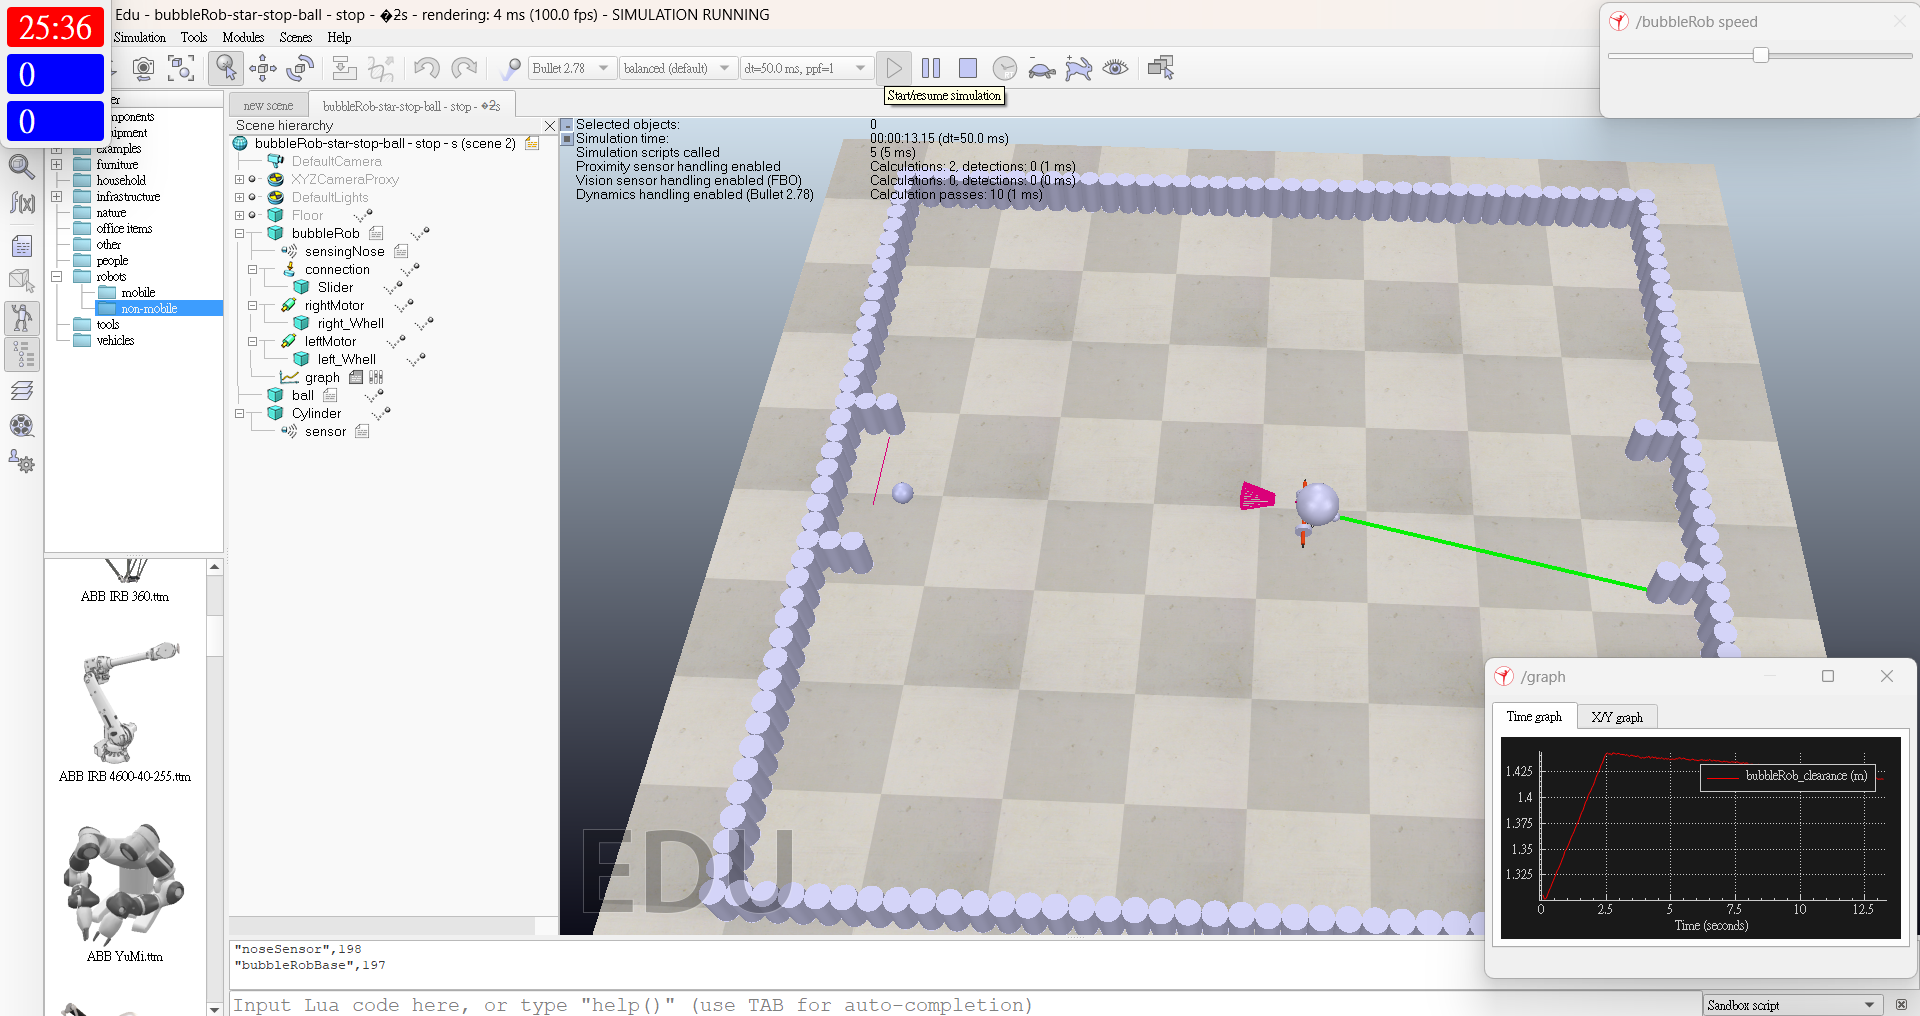
\includegraphics[width=16cm]{326}
\caption{\Large 記分板與計時 }\label{記分板與計時}
\end{center}
\end{figure} 
\qquad \\
\\
\\
使用了xml進行編寫,再利用simUI.create顯示出來\\
設定在不同的條件下,更改顯示的數字\\
倒數結束時則利用sim.stopSimulation()來停止模擬
\begin{figure}[hbt!]
\begin{center}
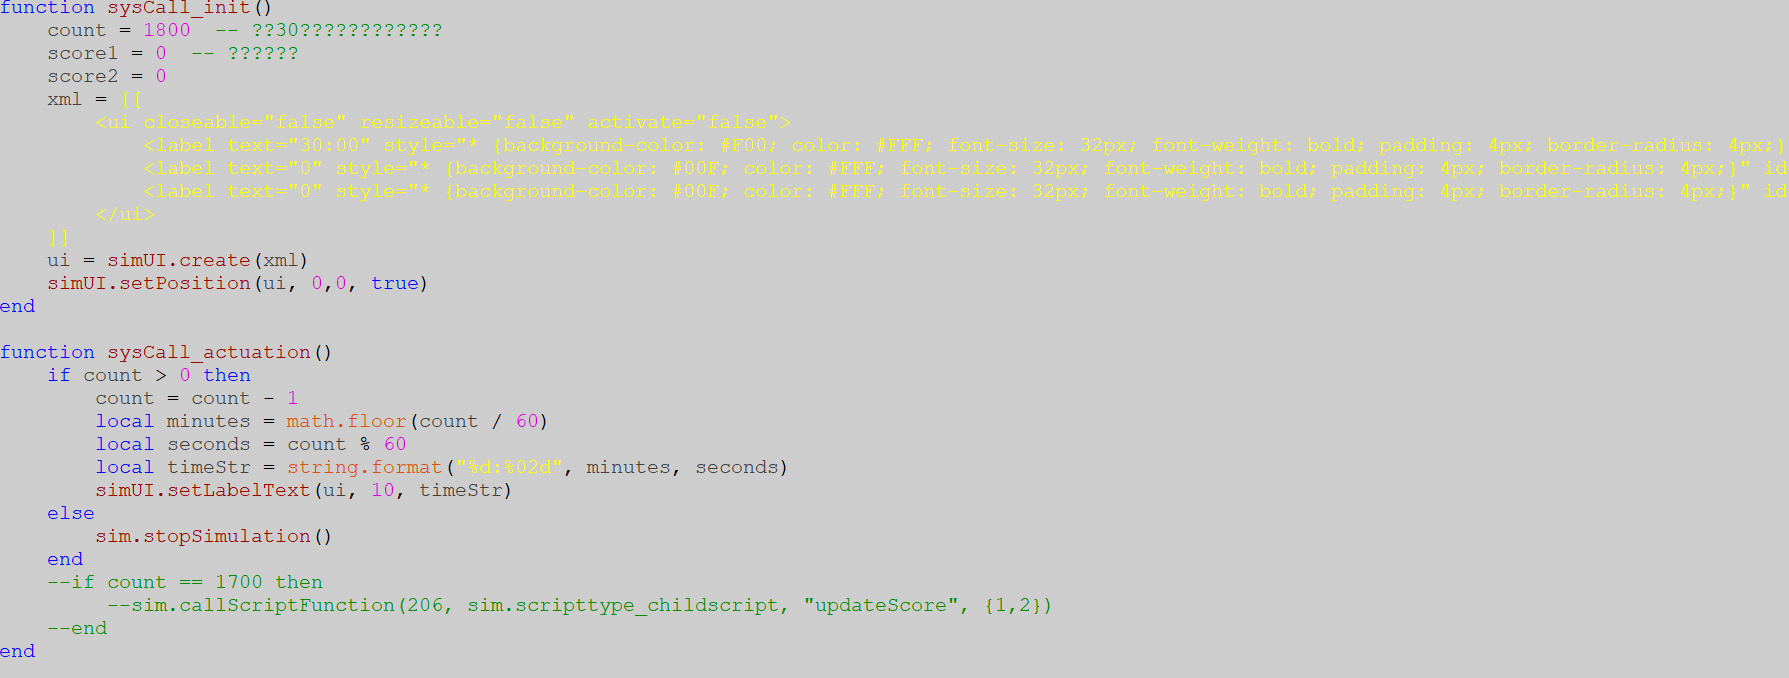
\includegraphics[width=16cm]{記分板與計時程式}
\caption{\Large 記分板與計時程式 }\label{記分板與計時程式}
\end{center}
\end{figure} 
\qquad \\
\\
\section{歡迎與恭喜}
%=--------------------歡迎與恭喜----------------------=%
加入了歡迎與得分的ui提升觀賞性,一樣使用xml編寫即可
使用同一個id,只是更改顯示的內容,開始時隱藏,暫停時顯現
\begin{figure}[hbt!]
\begin{center}
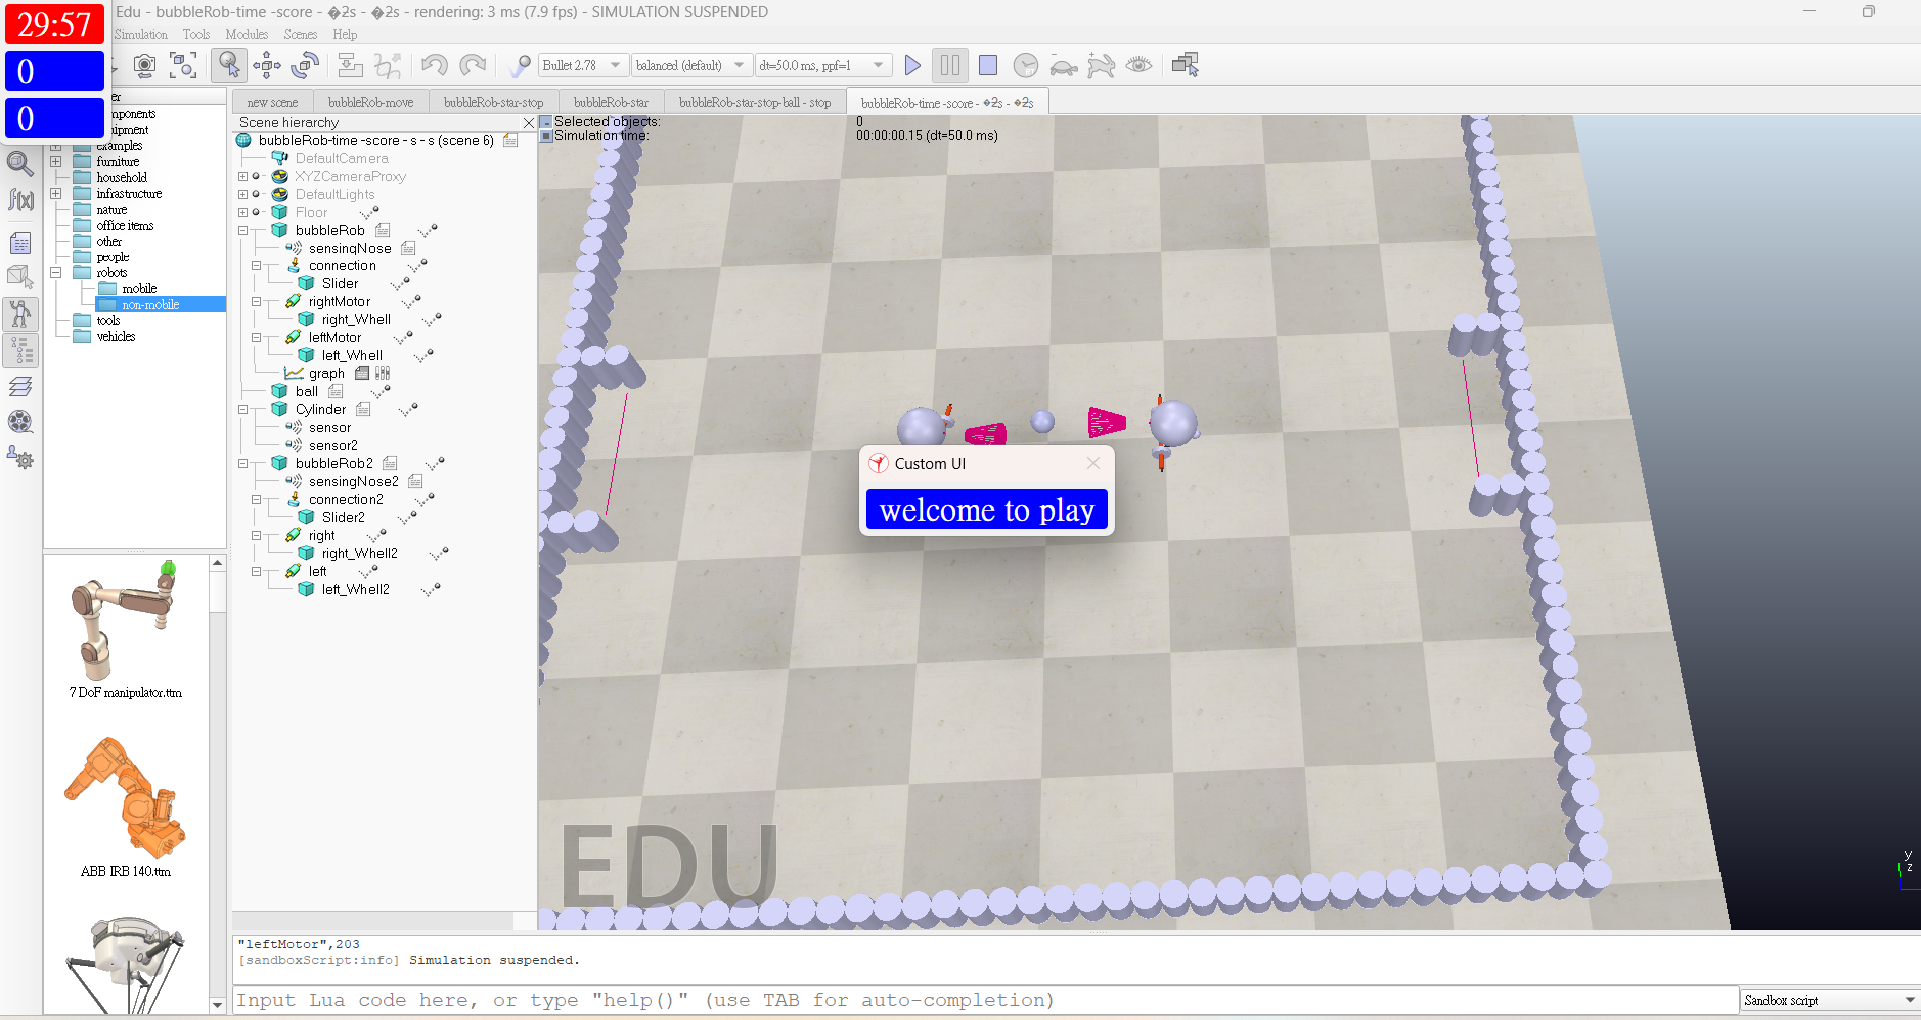
\includegraphics[width=16cm]{412-1}
\caption{\Large 歡迎 }\label{歡迎}
\end{center}
\end{figure} 
\qquad \\
\begin{figure}[hbt!]
\begin{center}
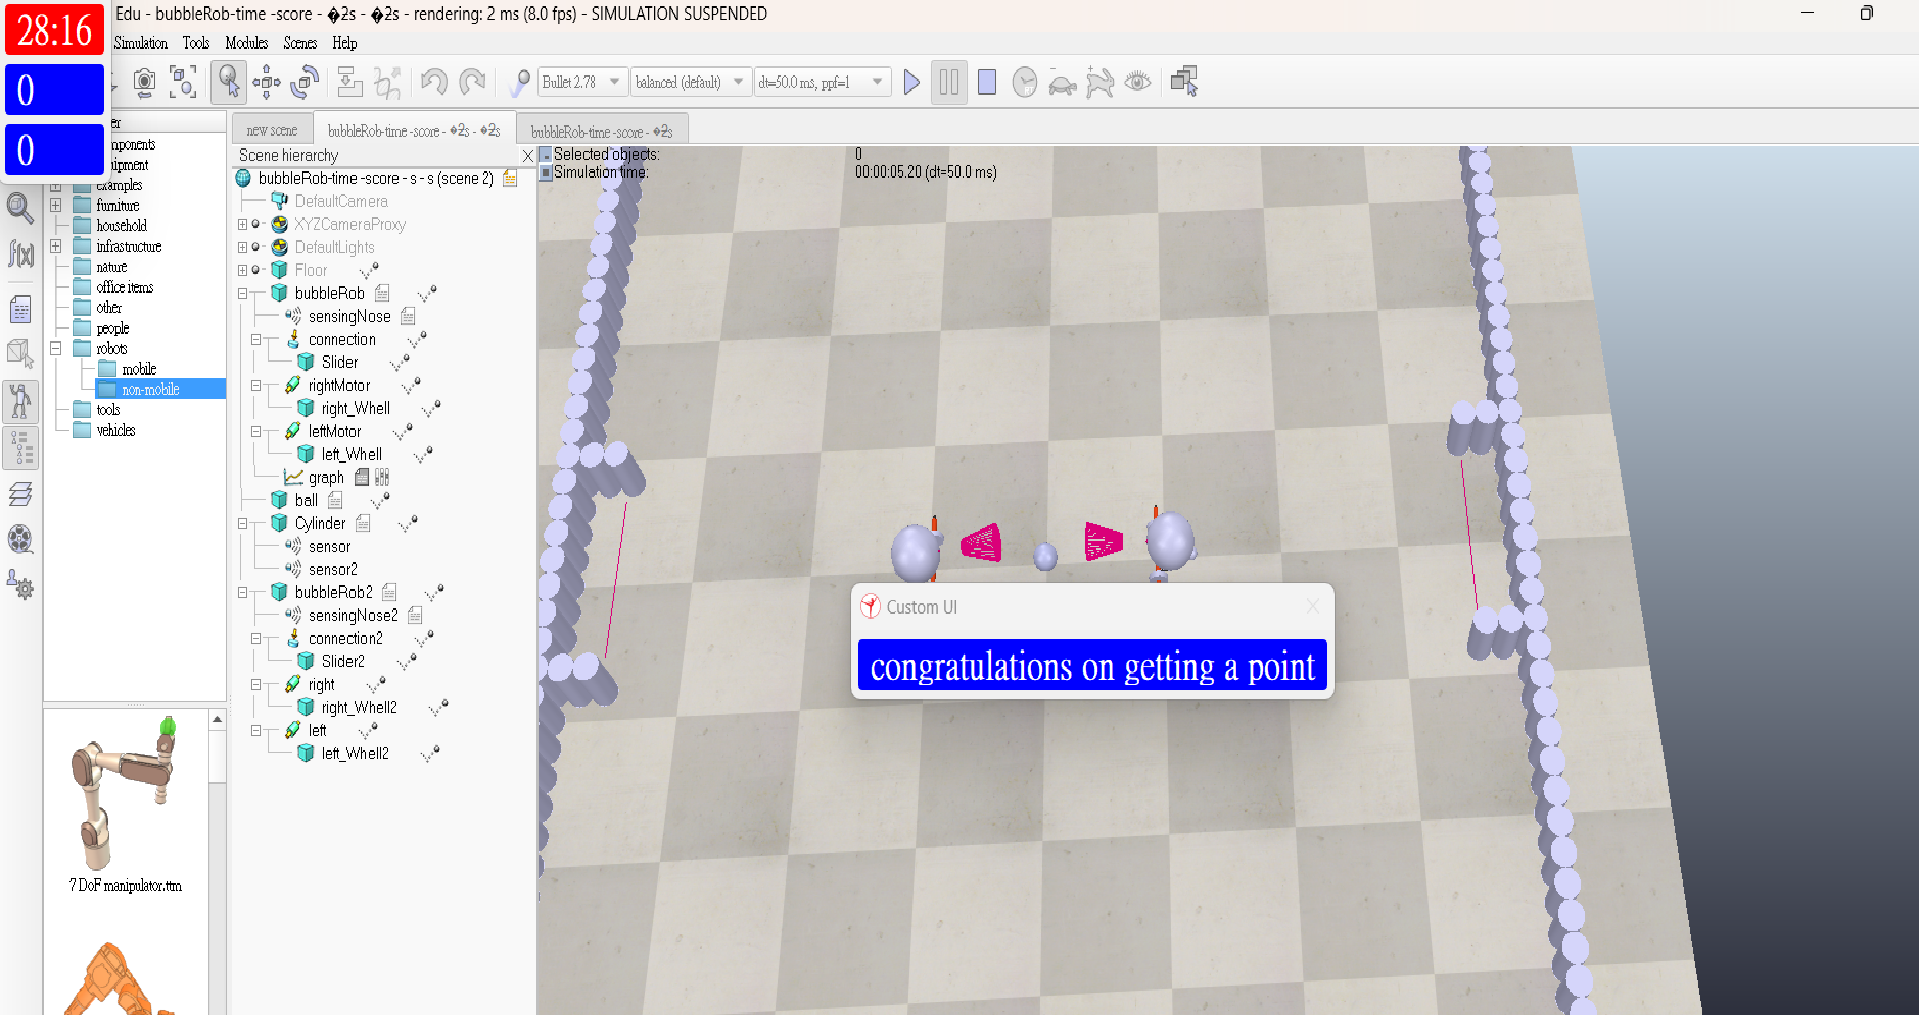
\includegraphics[width=16cm]{412-2}
\caption{\Large 恭喜 }\label{恭喜}
\end{center}
\end{figure} 
\qquad \\
\begin{figure}[hbt!]
\begin{center}
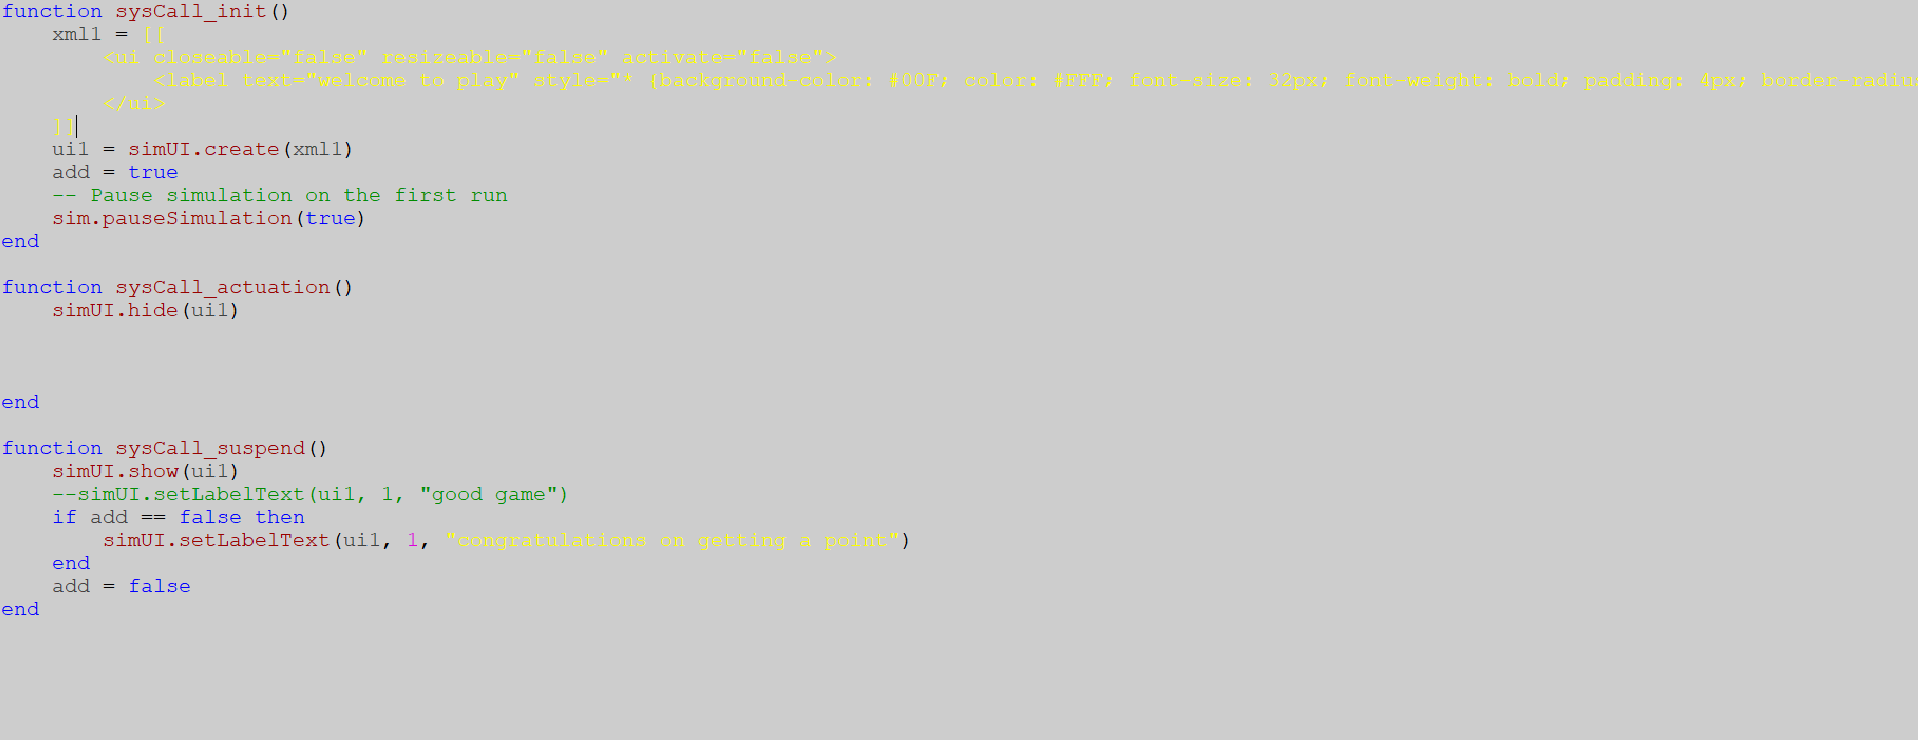
\includegraphics[width=16cm]{歡迎與恭喜lua}
\caption{\Large 歡迎與恭喜lua }\label{歡迎與恭喜lua}
\end{center}
\end{figure} 
\\
\section{RemoteApi}
%=--------------------RemoteApi----------------------=%
開啟19998與23020埠號來提供玩家使用RemoteApi連線
\begin{figure}[hbt!]
\begin{center}
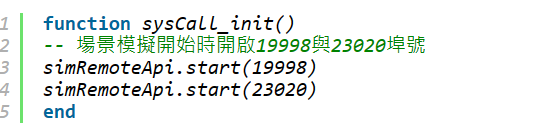
\includegraphics[width=16cm]{開啟埠號}
\caption{\Large 開啟埠號 }\label{開啟埠號}
\end{center}
\end{figure} 
\qquad \\
將前面使用lua編寫的控制移動程式轉為使用python編寫,並使用RemoteApi進行連線
在模擬未開啟前,可以使用19997默認埠號進行連線,須注意連線時coppeliasim畫面必須開啟\\
\begin{figure}[hbt!]
\begin{center}
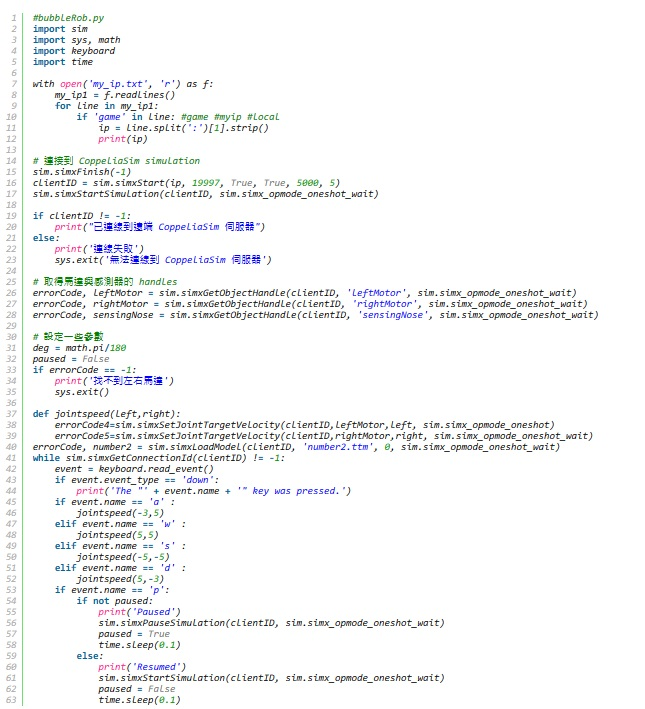
\includegraphics[width=16cm]{python操控}
\caption{\Large python操控 }\label{python操控}
\end{center}
\end{figure} 
\newpage